\section[Paramagnetism and Diamagnetism]{\hyperlink{toc}{Paramagnetism and Diamagnetism}}


\textbf{General}
\begin{itemize}
    \item original data storage devices
    \item only started to understand micro level after advent of QM
    \item goes past band structure
    \item treat interactions between particles
    \item interactions between spins are fundamental to current research: spintronics + quantum technologies using spins.
    \item phase transitions
\end{itemize}

\textbf{Spinors}

\begin{equation}
    \alpha \ket{\uparrow} + \beta \ket{\downarrow} = \begin{pmatrix}
    \alpha  \\ \beta
    \end{pmatrix}, \qquad |\alpha|^2 + |\beta|^2 = 1
\end{equation}
\begin{equation}
    S_z = \frac{1}{2} \hbar \sigma_z, \qquad \sigma_z = \begin{pmatrix} 1 & 0 \\ 0 & -1 \end{pmatrix}
\end{equation}

\textbf{Bloch sphere representation}
\begin{equation}
    \ket{\Psi} = \cos{\frac{\theta}{2}}\ket{\uparrow} + \sin{\frac{\theta}{2}}e^{i\phi}\ket{\downarrow}
\end{equation}

\textbf{Magnetic Susceptibility}
\begin{equation}
    M = \chi \frac{\textbf{B}}{\mu_0}
\end{equation}

 \begin{tcolorbox}[enhanced,attach boxed title to top center={yshift=-3mm,yshifttext=-1mm},
  colback=blue!5!white,colframe=blue!75!black,colbacktitle=red!80!black,
  title=Bohr-van Leeuwen Theorem,fonttitle=\bfseries,
  boxed title style={size=small,colframe=red!50!black} ]
  \begin{equation}
      \braket{\textbf{M}} = \braket{\lambda \textbf{L}} = 0, \qquad \text{according to classical statistics} \rightarrow \text{magnetism obeys quantum statistics}
  \end{equation}
\end{tcolorbox}

\textbf{Properties of Magnetism can have three origins,}
\begin{itemize}
    \item Intrinsic angular momentum (Spin). 
    \item Orbital angular momentum about the nuleus
    \item Change in the dipole moment due to an applied magnetic.
    
    \item When electrons are \textbf{paired together} their opposite spins cause their magnetic fields to cancel each other. Therfore, \textbf{no net magnetic field exists}. Alternatively, materials with some \textbf{unpaired electrons} will have a \textbf{net magnetic field} and will \textbf{react} more to an \textbf{external field}.
\end{itemize}

\textbf{Hund's Rules (L-S coupling scheme -- how to fill up orbitals in atoms):}
\begin{itemize}
    \item Outer shell electrons of an atom in its ground state should assume:
    \begin{enumerate}
        \item Max Value of S (spin momentum) allowed by exclusion princple.
        \item Maximum value of L (orbital momentum) compatible with (1).
        \item $J=|L-S|$ for less than half-filled shells. \\$J = L+S$ for more than half-filled shells.
        
        Causes: 
        $
        \begin{cases}
        \text{parallel spins have lower Coulomb energy.}\\
        \text{e's meet less frequently if orbiting in same direction (parallel Ls).} \\
        \text{Spin orbit coupling lowers energy for} + L*S < 0
        \end{cases}
        $
    \end{enumerate}
    
    \item examples:\\
    $
    \begin{cases}
    \text{Mn}^{2+}: \qquad 3d^5 \qquad (1) \rightarrow S=5/2 \qquad \text{excl. princ.} \rightarrow L = 2+1+0-1-2 = 0 \\
    \text{Ce}^{3+}:\qquad 4f^1 \qquad L = 3, S = \frac{1}{2} \qquad (3) \rightarrow J = |3-\frac{1}{2}| = 5/2 \\
    \text{Pr}^{3+}: \qquad 4f^2
    \qquad (1) \rightarrow S = 1 \qquad (2) \rightarrow L = 3+2 = 5 \qquad (3) \rightarrow J = |5-1|=4
    \end{cases}
    $
    \item shell filling structure is important
\end{itemize}

\textbf{Paramagnetism (positive suceptibility):}
\begin{itemize}
    \item a paramagnet has a response that tends to enhance the applied field, i.e., \textbf{$\chi > 0.$}
    \item This is usually due to the spin of the \textbf{unpaired electrons} fixed within the crystal.
    \item the simplest model for p.m. (known as \textbf{Currie Paramagnetism} after Pierre Curie, or Langevin Paramagnetism) is the result of considering a collection of non-interacting spin-1/2 particles.
    \item Occurence of electronic paramagnetism:
    \begin{itemize}
        \item Atoms, molecules, and lattice defects with \textbf{odd numbers of electrons} (S $\neq$ 0).
        E.g., Free sodium atoms, gaseous NO, F centers in alkali halides, organic free radicals such as $C(C_6H_5)_3$
        \item Free atoms and ions with \textbf{partly filled inner shell} (free or in solid), E.g., Transition elements, ions isoelectronic with transition elements, rare earth and actinide elemnts such as $\text{Mn}^{2+}\text{, Gd}^{3+}\text{, U}^{4+}.$
        \item Only a few compounds with even number of electrons, E.g. $O_2$, organic biradicals.
        \item \textbf{metals}
    \end{itemize}
    \item For a free spin-1/2 particle, the Hamiltonian is given by the so called the Zeeman Term:
    \[ H = g \mu_B \textbf{B}\cdot \vec{\sigma} \]
    where $g=2$ is the g-factor for the electron, $\vec{\sigma}$ is an operator for the spin and $\mu_B = e\hbar/(2m) \approx 0.67k_B $ Kelvin/Tesla is the Bohr Magneton.
    \item The single spin can be oriented either parallel or antiparallel to the field, so the energies for the two states of a single spin can be:
    \[ E = \pm \mu_B B \]
    \item Then we know that the probabilities of the two states are given by:
    \[p_{\uparrow} = \frac{e^{-\beta \mu_B B}}{Z}, \qquad  p_{\downarrow} = \frac{e^{+\beta \mu_B B}}{Z}, \qquad Z = e^{-\beta \mu_B B}+ e^{+\beta \mu_B B}\]
    where $\beta = 1/(k_B T) $
    \item Zeeman Splitting
    \item 36:00min derivation to get susceptibility:
    \[ \chi = \frac{\mu_0 \mu_B^2}{k_B T}\]
    and for a collection of spins with density n we then have 
    \[\chi = \frac{n \mu_0 \mu_B^2}{k_B T} \]
    \item Result: \textbf{Magnetization increases as you lower the temperature: Currie Law susceptibility is dependence on $1/T$}
\end{itemize}

\textbf{Paramagnetic Susceptibility of Conduction Electrons:}
\begin{itemize}
    \item Classical free electrons: $M \approx \frac{N \mu^2 B}{k_B T} \qquad \sim$ Curie paramagnetism
    
    \item Experiments on normal non-ferromagnetic metals: M independent of T
    
    \item Pauli's resolution: Electrons in Fermi sea cannot flip over due to exclusion principle. Only fraction $T/T_f$ near Fermi level can flip.
\end{itemize}

\textbf{Pauli Paramagnetism}
\begin{itemize}
    \item For some alkali metals and noble metals, conduction electrons are weakly interacting and delocalized in space forming a Fermi gas. For these materials one contribution to the magnetic response comes from the interaction between the electron spins and the magnetic field known as Pauli paramagnetism. 
    \item The Pauli paramagnetic susceptibility is a macroscopic effect and has to be contrasted with Landau diamagnetic susceptibility which is equal to minus one third of Pauli's and also comes from delocalized electrons. The Pauli susceptibility comes from the spin interaction with the magnetic field while the Landau susceptibility comes from the spatial motion of the electrons and it is independent of the spin. In doped semiconductors the ratio between Landau's and Pauli's susceptibilities changes as the effective mass of the charge carriers $m^{*}$ can differ from the electron mass $m_{e}$.
    
    \item Before Pauli's theory, the lack of a strong Curie paramagnetism in metals was an open problem as the leading Drude model could not account for this contribution without the use of quantum statistics. Pauli paramagnetism and Landau diamagnetism are essentially applications of the spin and the free electron model, the first is due to intrinsic spin of electrons the second is due to their orbital motion.
\end{itemize}

\textbf{Diamagnetism}
\begin{itemize}
    \item can come from orbital mechanism in a Free Electron Gas (not going to talk much about it)
    \item or from a fully filled shell
    \item famous example is frog floating in a magnetic field (diamagnetism)
    \item phenom characterized by negative susceptibility ($\chi<0$).
    \item appears in most materials but is often dominated by other effects
    \item superconductors tend to be good diamagnets
    \item main type is called Larmor diamagnetism (comes from Larmor Precession) when other magnetic effects are not present.
    \item Need J=0 otherwise Curie Paramagnetism dominates
    \item relates in Lenz's Law
    \item you can also use paramagnets to make an adiabatic demagnetization refrigerators
\end{itemize}


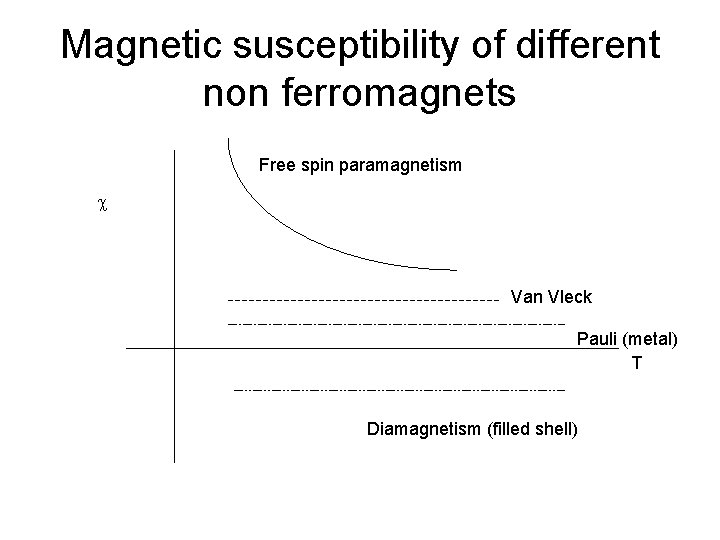
\includegraphics[width = \linewidth]{Images/paramagnetism.jpg}

